\begin{frame}
	\frametitle{Git}
	\begin{block} <1-> {Eigenschaften}
		\begin{itemize}
			\item <1-> Dezentralität
			\begin{itemize}
				\item <1-> klon des kompletten Repositories lokal
			\end{itemize}
			\item <2-> Vieles läuft lokal
			\item <3-> Hashes statt Nummern
			\begin{itemize}
				\item <3-> dezentrale Architektur erlaubt keine fortlaufende Revisiond-Nummerierung
			\end{itemize}
			\item <4-> Lizenz: GNU GPLv2 (Frei Software / Open-Source-Software)
		\end{itemize}
	\end{block}
\end{frame}
\begin{frame}
	\frametitle{Git}
	\framesubtitle{4 Ebenen}
	\begin{columns}
		\column{0.5\textwidth}
			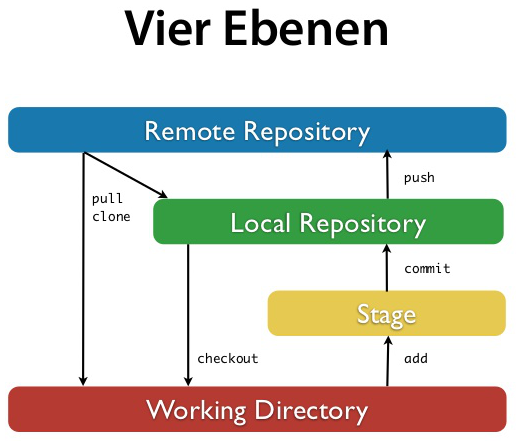
\includegraphics[scale=0.45]{./pictures/4_ebenen_git}
		\column{0.5\textwidth}
			\begin{block} <2-> {Remote Repository}
				Versionen des Projektes, welche sich im Internet oder Netzwerk befindet.
			\end{block}
			\begin{block} <3-> {Local Repository}
				Versionen des Projektes, welche sich lokal auf dem System befinden. 
			\end{block}
			\begin{block} <5-> {Stage}
				Eine Zwischenablage, aus der herraus man committen kann.
			\end{block}
			\begin{block} <4-> {Working Directory}
				Die eigentlichen Dateien
			\end{block}
	\end{columns}
\end{frame}